\documentclass[a4paper]{article}
\addtolength{\hoffset}{-2.25cm}
\addtolength{\textwidth}{4.5cm}
\addtolength{\voffset}{-3.25cm}
\addtolength{\textheight}{5cm}
\setlength{\parskip}{0pt}
\setlength{\parindent}{0in}

%----------------------------------------------------------------------------------------
%	PACKAGES AND OTHER DOCUMENT CONFIGURATIONS
%----------------------------------------------------------------------------------------

\usepackage{blindtext} % Package to generate dummy text
\usepackage{charter} % Use the Charter font
\usepackage[utf8]{inputenc} % Use UTF-8 encoding
\usepackage{microtype} % Slightly tweak font spacing for aesthetics
\usepackage[english, ngerman]{babel} % Language hyphenation and typographical rules
\usepackage{amsthm, amsmath, amssymb} % Mathematical typesetting
\usepackage{float} % Improved interface for floating objects
\usepackage[final, colorlinks = true, 
            linkcolor = black, 
            citecolor = black]{hyperref} % For hyperlinks in the PDF
\usepackage{graphicx, multicol} % Enhanced support for graphics
\usepackage{xcolor} % Driver-independent color extensions
\usepackage{marvosym, wasysym} % More symbols
\usepackage{rotating} % Rotation tools
\usepackage{censor} % Facilities for controlling restricted text
\usepackage{listings, style/lstlisting} % Environment for non-formatted code, !uses style file!
\usepackage{pseudocode} % Environment for specifying algorithms in a natural way
\usepackage{style/avm} % Environment for f-structures, !uses style file!
\usepackage{booktabs} % Enhances quality of tables
\usepackage{tikz-qtree} % Easy tree drawing tool
\tikzset{every tree node/.style={align=center,anchor=north},
         level distance=2cm} % Configuration for q-trees
\usepackage{style/btree} % Configuration for b-trees and b+-trees, !uses style file!
\usepackage[backend=biber,style=numeric,
            sorting=nyt]{biblatex} % Complete reimplementation of bibliographic facilities
\addbibresource{ecl.bib}
\usepackage{csquotes} % Context sensitive quotation facilities
\usepackage[yyyymmdd]{datetime} % Uses YEAR-MONTH-DAY format for dates
\renewcommand{\dateseparator}{-} % Sets dateseparator to '-'
\usepackage{fancyhdr} % Headers and footers
\pagestyle{fancy} % All pages have headers and footers
\fancyhead{}\renewcommand{\headrulewidth}{0pt} % Blank out the default header
\fancyfoot[L]{} % Custom footer text
\fancyfoot[C]{} % Custom footer text
\fancyfoot[R]{\thepage} % Custom footer text
\newcommand{\note}[1]{\marginpar{\scriptsize \textcolor{red}{#1}}} % Enables comments in red on margin

%----------------------------------------------------------------------------------------

\begin{document}

%-------------------------------
%	TITLE SECTION
%-------------------------------

    \fancyhead[C]{}
    \hrule \medskip % Upper rule
    \begin{minipage}{0.295\textwidth}
        \raggedright
        \footnotesize
        \textbf{Pedro Luis Lobato Barros} \hfill\\
        202012490\hfill\\
        p.lobato

        \textbf{Jaime Andres Torres Bermejo} \hfill\\
        202014866\hfill\\
        j.torres16

        \textbf{Sofia Torres Ram\'irez} \hfill\\
        202014872\hfill\\
        s.torres21

    \end{minipage}
    \begin{minipage}{0.4\textwidth}
        \centering
        \large
        Caso 1\\
        \normalsize
        Infraestructura Computacional - Universidad de los Andes\\
    \end{minipage}
    \begin{minipage}{0.295\textwidth}
        \raggedleft
        \today\hfill\\
    \end{minipage}
    \medskip\hrule
    \bigskip

%-------------------------------
%	CONTENTS
%-------------------------------


    \section{Estructura del Proyecto}

    \subsection{UML}
    \begin{center}
        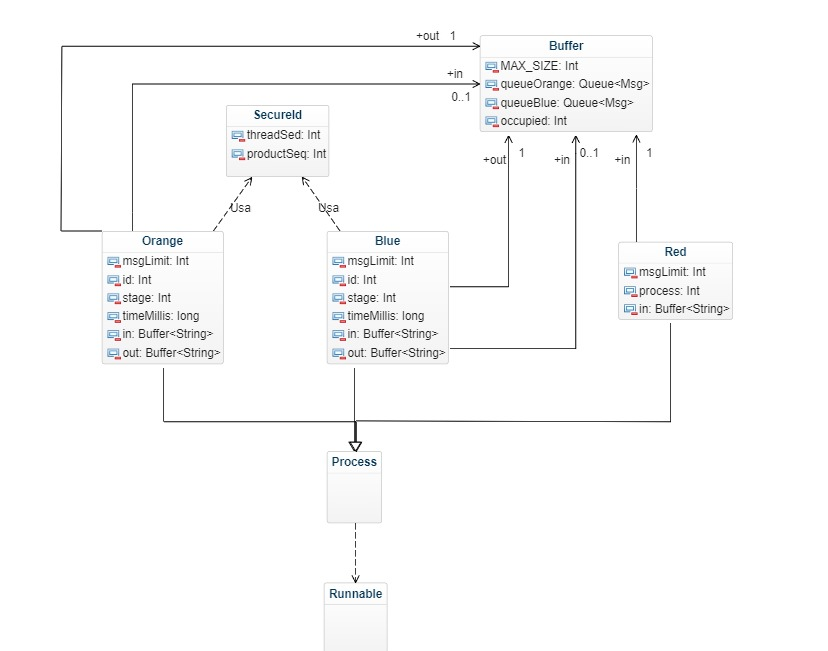
\includegraphics[scale=0.5]{uml.jpeg}    
    \end{center}
    
    Por medio de este diagrama UML se puede entender a grandes rasgos el funcionamiento del programa.
    Iniciando por la clase \code{Process} podemos ver que esta clase extiende de \code{Runnable} en pro de seguir el lenguaje manejado en el caso.
    Siguiendo con esta idea se aprecian las clases \code{Orange}, \code{Blue} y \code{Red} que representan los diferentes procesos que puede tener el programa, para eso cada uno implementar\'a la interfaz \code{Process}.\\
    Tal como lo evidencia el diagrama, las clases que implementan a \code{Process} tienen el objetivo de interactuar con procesos (Creando, transformando o envi\'andolos).
    Sin embargo, su funcionamiento interno es diferente y este ser\'a especificado en la secci\'on 1.3.\\
    Los atributos que los tipos de procesos comparten son:
    \begin{itemize}
        \item \code{String msgLimit}: El n\'umero de productos o mensajes que se deben crear por cada tipo de proceso y que por ende se deben imprimir al finalizar el programa.
        Este atributo es est\'atico, por lo tanto, est\'a subrayado.
        \item \code{int id}: El identificador de cada proceso creado.*
        \item \code{int stage}: El identificador de la etapa en la cual se encuentra el proceso creado.*
        \item \code{long timeMillis}: El tiempo que debe dormir el proceso para simular la modificaci\'on del mensaje/producto.*
        \item \code{Buffer in}: El buz\'on de entrada del proceso (explicado m\'as adelante).
        \item \code{Buffer out}: El buzo\'on de salida del proceso (explicado m\'as adelante).*
        \item[\textbullet] \code{int process}: La cantidad de procesos por etapa.
    \end{itemize}
    \small{* \code{Red} no posee estos atributos marcados por su posici\'on al final del todo y por el hecho que no necesita transformar el mensaje.}\\
    \small{\textbullet \code{Red} es el \'unico tipo de proceso con este atributo; atributo necesario para saber cuando finaliza la ejecuci\'on.}

    Con respecto a la clase \code{Buffer} podemos ver que tiene los siguientes atributos:
    \begin{itemize}
        \item \code{int MAX\_SIZE}: La capacidad del buffer.
        \item \code{Queue queueOrange}: Una cola que almacena los productos/mensajes que fueron creados y modificados por procesos naranjas.
        \item \code{Queue queueBlue}: Una cola que almacena los productos/mensajes que fueron creados y modificados por procesos azules.
        \item \code{int occupied}: La cantidad de productos/mensajes que hay en el buffer.
    \end{itemize}

    Tanto el proceso naranja (Orange) como el azul (Blue) tienen dos relaciones con el Buffer.
    El hecho que la relaci\'on con el buz\'on de entrada posea una cardinalidad de 0..1 est\'a relacionado a la etapa del proceso en si, si se es la etapa inicial no hay producto que ``sacar'' pero si un mensaje que producir.
    Para el resto de etapas ya hay un producto que ``sacar''.\\
    Por otro lado, para todo proceso azul o naranja siempre existir\'a un buz\'on de salida en el cual se colocan los mensajes ya modificados o reci\'en generados para que un proceso de la siguiente etapa pueda interactuar con el producto.\\
    Sin embargo, el proceso rojo no funciona igual debido a que este proceso solo tendr\'a interacci\'on con el \'ultimo buz\'on, del cual sacar\'a la totalidad de mensajes para luego imprimirlos.

    \subsection{Main.java}

    \subsubsection{La interfaz \code{Process}}
    Su \'unico objetivo es el de estipular que los otros tipos de procesos son\ldots Procesos, en otras palabras es una decisi\'on tomada para que se apegue al lenguaje del caso.

    \subsubsection{La clase \code{SecureId}}
    Su objetivo es el de otorgar las ids necesarias para seguir el proceso de los mensajes y procesos.
    Para cumplir esa funci\'on est\'an sus atributos est\'aticos:
    \begin{itemize}
        \item \code{int threadSeq}: Para identificar a los hilos (procesos).
        \item \code{int productSeq}: Para identificar a los mensajes.
    \end{itemize}

    \subsubsection{La clase \code{Main}}
    La principal funci\'ion de la clase \code{Main}, adem\'as de correr el programa,
    es preparar al resto del programa para su funcionamiento \'optimo.\\

    Una de las primeras cosas que van a saltar a la vista es el uso de variables
    definidas con el estado de \code{final} dentro de la propia l\'ogica de java.
    Con esto, se pretende hacer que las variables definidas sean inmutables y no puedan ser alteradas una vez definidas ni por el usuario ni por ninguno de los procesos que el programa corra.
    Las variables que caen dentro de este conjunto inmutable son:
    \begin{itemize}
        \item \code{int MESSAGE\_NUM}: Define el n\'umero de mensajes a enviar.
        \item \code{int PROCESS\_NUM}: Define el n\'umero de procesos del programa.
        \item \code{int BUFFER\_CAP}: Define el l\'imite del Buffer
        \item \code{int BUFFER\_NUM}: Define el n\'umero de Buffers
        \item \code{int STAGE\_NUM}: Define el n\'umero de etapas por las que pasar\'an los procesos
    \end{itemize}

    Estas constantes son luego utilizadas para la creaci\'on de los objetos que ser\'an usados en el programa, y conectar\'a la l\'ogica de esos nuevos objetos creados.

    \subsection{Estructura de los Procesos}

    \subsubsection{Blue}
    \begin{center}
        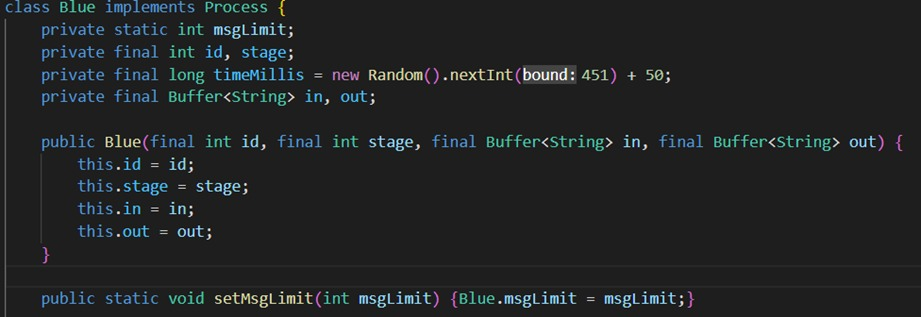
\includegraphics[scale=0.5]{B1.jpeg}    
    \end{center}
    En la parte inicial del c\'odigo se puede ver la definici\'on de los atributos de la clase \code{Blue}, su m\'etodo constructor y el setter para el atributo est\'atico \code{msgLimit}.
    Luego de esto podemos ver el m\'etodo run del proceso, en donde, si la etapa del proceso creado es igual a 0, correr\'a el m\'etodo \code{runZero( )}; de lo contrario, correr\'a el m\'etodo \code{runNonZero( )}.
    Esto se hace debido a que, si el proceso pertenece a la etapa cero, quiere decir que a\'un no se han producido los productos/mensajes, por ende, toca crearlos.
    Si la etapa es diferente de 0, ya est\'an generados los mensajes as\'i que el proceso deber\'ia obtenerlos del buffer de entrada.
    
    \paragraph{M\'etodo \code{runZero( )}}
    \begin{center}
        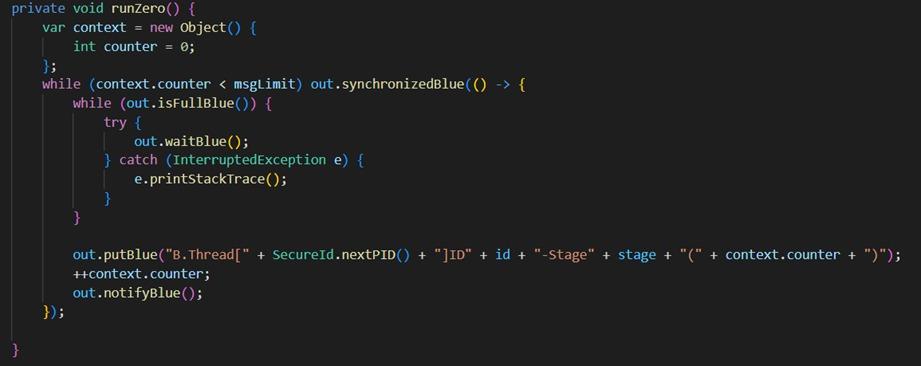
\includegraphics[scale=0.5]{B2.jpeg}    
    \end{center}
    En este m\'etodo se vale de un objeto an\'onimo para poder interactuar adecuadamente con la expresi\'on lambda que se encuentra m\'as adelante, dicho objeto contiene al atributo \code{counter} que servir\'a para saber cuando se ha llegado al l\'imite de los mensajes con los que debe interactuar el proceso.
    Prosiguiendo se destaca un while que verifica lo mencionado en la explicaci\'on anterior relacionada al l\'imite de mensajes para estar inmediatamente continuado por un m\'etodo que se vale de la expresi\'on lambda o funci\'on an\'onima.
    (La forma en que se maneja ser\'a explicada m\'as adelante).
    Siguiendo se encuentra la parte del c\'odigo encargada de asignar la espera pasiva para los procesos azules y la creaci\'on de los productos mientras haya espacio para finalizar ubicando el mensaje en el buz\'on, aumentando el contador de \code{counter} y notificando a alg\'uno de los hilos que interact\'uan con ese buz\'on.
    \pagebreak
    \paragraph{M\'etodo \code{runNonZero( )}}
    \begin{center}
        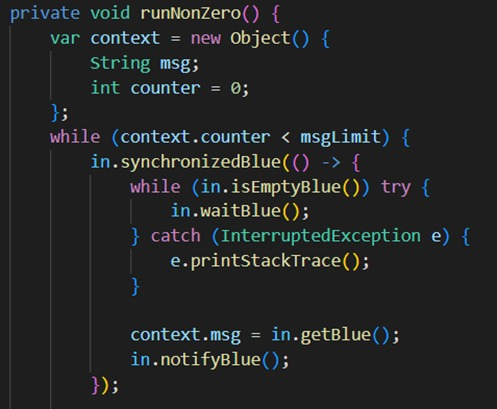
\includegraphics[scale=0.5]{B3.jpeg}    
    \end{center}
    Por otra parte, este m\'etodo tiene un comportamiento similar al anterior:
    Para la secci\'on de obtener hay una variaci\'on representada sobre \textbf{que} objeto se aplica la sincronizaci\'on y la condici\'on ahora es para comprobar si est\'a vac\'io.\\
    Por otra parte, la secci\'on de poner solo presenta la variaci\'on que pone el mensaje ya transformado en lugar de uno creado.
    Aclarando, se ejecuta un ciclo en donde, si la cola de mensajes azules del buffer de salida est\'a lleno, se notifica que se est\'a intentando agregar un nuevo mensaje a la cola y luego espera a que haya espacio en ella para poder agregar el mensaje.
    Cuando la cola no est\'a llena se agregar\'a el mensaje modificado y el contador de mensajes procesados aumenta en uno.
    Luego de esto, se notifica a todos los que est\'en esperando sobre esta cola por si alg\'un proceso de la siguiente etapa estaba esperando por \'el.
    No se realiza un \code{notify( )} debido a que es posible que se notifique a un proceso que ya haya terminado de procesar sus mensajes.\\
    Nota: Para cumplir lo anterior se sigue valiendo de la expresi\'on lambda.\\
    Entre ambas secciones mencionadas se ejecuta la transformaci\'on necesaria del mensaje agreg\'andole esta nueva etapa por la que pas\'o y luego el proceso se duerme por un tiempo aleatorio simulando el tiempo que toma dicha transformaci\'on.

    \subsubsection{Orange}
    
    \begin{center}
        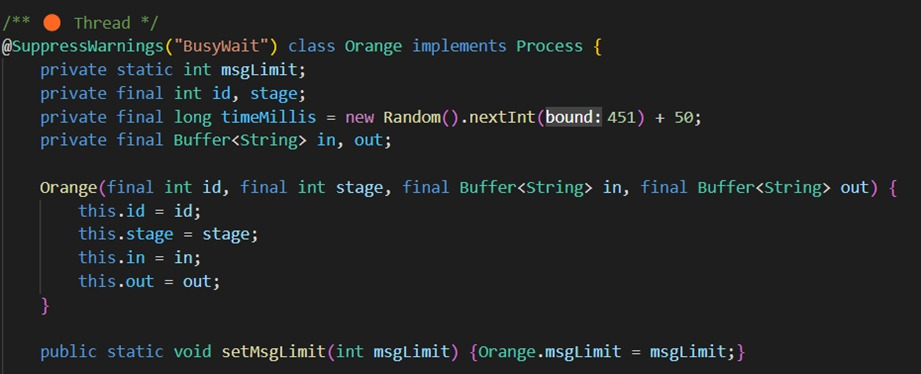
\includegraphics[scale=0.5]{N0.jpeg}    
    \end{center}

    En resumen se sigue la estructura del azul, pero con la variaci\'on que en la secci\'on de la expresi\'on lambda ahora usa dos fragmentos de c\'odigo para separar la parte no sincronizada de la sincronizada (Mejor explicado en la secci\'on dedicada a la clase \code{Buffer}).\\
    Ahora ahondando m\'as: En la parte inicial del c\'odigo se puede ver la definici\'on de los atributos de la clase Orange, su m\'etodo constructor y un m\'etodo para darle valor al atributo \code{msgLimit}.
    Luego de esto podemos ver el m\'etodo run del proceso en donde, si la etapa del proceso creado es igual a 0, correr\'a el m\'etodo \code{runZero( )}, de lo contrario correr\'a el m\'etodo \code{runNonZero( )}. Esto se hace debido a que, si el proceso pertenece a la etapa cero, quiere decir que a\'un no se han creado los productos/mensajes, por ende, toca crearlos. Si la etapa es diferente de 0, ya est\'an creados los mensajes as\'i que el proceso tendr\'ia que obtenerlos del buffer de entrada.

    \begin{center}
        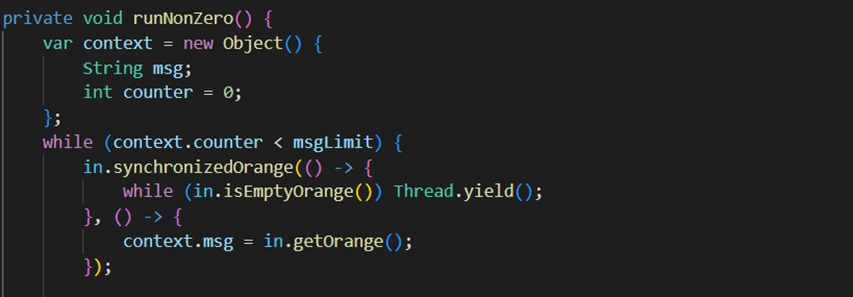
\includegraphics[scale=0.5]{N1.jpeg}    
    \end{center}
    En la primera parte del m\'etodo \code{runNonZero( )} se crea un objeto an\'onimo \code{context} el cu\'al tendr\'a dos atributos \code{msg} y \code{counter}, en donde \code{msg} ser\'a el mensaje sacado del buffer de entrada y \code{counter} ser\'a el n\'umero de mensajes que se han procesado.
    Teniendo en cuenta esta informaci\'on, luego se ejecutar\'a un ciclo mientras todav\'ia no se hayan procesado todos los mensajes azules.
    Siguiente a esto se llama a la m\'etodo \code{in.synchronizedOrange( )} la cu\'al permite la distinci\'on entre bloques, en el primer bloque de instrucciones a\'un no se sincroniza respecto a la cola de mensajes naranjas del buffer, mientras que en el segundo s\'i exista esta sincronizaci\'on.
    En el primer bloque se eval\'ua si la cola de mensajes naranjas est\'a vac\'ia.
    Si esto es cierto, se ejecuta la instrucci\'on \code{Thread.yield( )} la cual generar\'a que el proceso ceda el procesador y lo vuelva a solicitar inmediatamente para volver a consultar hasta que ya no est\'e vac\'ia.
    Es aqu\'i en donde se puede evidenciar el comportamiento de espera semi-activa por parte del proceso naranja y tambi\'en se identifica la importancia de dejar la instrucci\'on del \code{yield} por fuera de la sincronizaci\'on del recurso para no generar un \texttt{deadlock}.
    Cuando la cola de mensajes naranjas ya no est\'a vac\'ia se ejecuta el segundo bloque del m\'etodo \code{in.synchronizedOrange( )} lo que quiere decir que en esta parte del c\'odigo s\'i se estar\'a sincronizando respecto a la cola de mensajes naranjas.
    En esta parte del c\'odigo se tomar\'a un mensaje de la cola de mensajes naranjas para luego liberar al recurso.
    Es decir, ya no se sincroniza la cola.\\

    En la siguiente parte del c\'odigo se realiza la transformaci\'on necesaria del mensaje agreg\'andole esta nueva etapa por la que pas\'o y luego el proceso se duerme por un tiempo aleatorio simulando dicha transformaci\'on.
    Luego de modificar el mensaje es necesario agregarlo al buffer de salida (out) debido a esto, primero se llama a la funci\'on \code{out.synchronizedOrange( )} (Cuyo funcionamiento ya ha sido explicado).
    El primer bloque de este m\'etodo ser\'a ejecutar un ciclo en donde si la cola de mensajes naranjas del buffer de salida est\'a llena, se hace \code{Thread.yield( )} en donde el proceso naranja ceder\'a el procesador y lo volver\'a a solicitar inmediatamente hasta que la cola ya no est\'e llena.
    Luego, en el segundo bloque de en el cual se sincronizar\'a la cola de mensajes naranjas del buffer de salida, cuando la cola no est\'e llena se agregar\'a el mensaje modificado y el contador de mensajes procesados aumentar\'a en uno.\\


    \begin{center}
        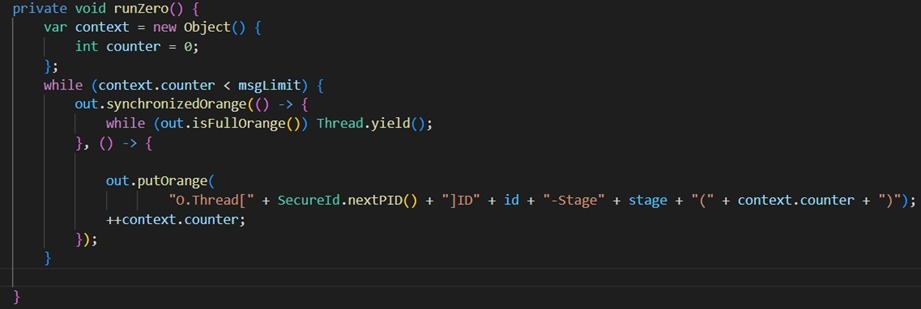
\includegraphics[scale=0.5]{N2.jpeg}    
    \end{center}
    Por \'ultimo se tiene el m\'etodo \code{runZero( )} en donde se crea un objeto an\'onimo \code{context} el cual tiene un atributo llamado \code{counter} que cuenta la cantidad de productos/mensajes creados.
    Luego de esto se ejecuta un ciclo mientras el n\'umero de mensajes producidos sea menor al n\'umero de mensajes a crear.
    Mientras esto suceda se har\'a uso del m\'etodo \code{out.synchronizedOrange( )} (Con su funcionamiento ya explicado previamente) en donde el primer bloque de la funci\'on se evaluar\'a si la cola de mensajes naranjas del buffer de salida est\'a llena, de ser as\'i se ejecuta la instrucci\'on \code{yield} hasta que la cola de mensajes naranjas no est\'e llena.
    En el segundo bloque de la funci\'on, cuando esta cola ya no est\'a llena, se crea el mensaje, se agrega a la cola y luego se aumenta el contador de mensajes creados en uno.

    \subsubsection{Red}
    \begin{center}
        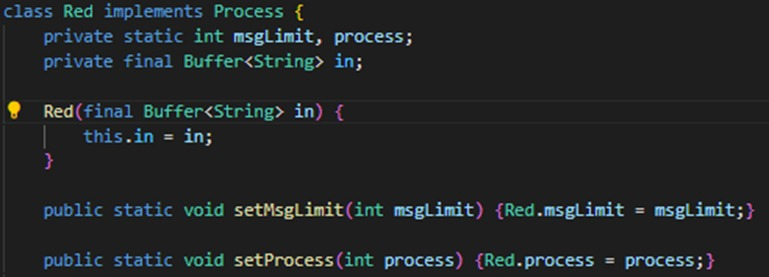
\includegraphics[scale=0.5]{R0.jpeg}    
    \end{center}
    En la parte inicial del c\'odigo se puede ver la definici\'on de los atributos de la clase Red, y los m\'etodos para darle valor a estos atributos.
    Adicionalmente, se puede la inicializaci\'on del m\'etodo \code{run( )} y dentro \'el la creaci\'on de variables de control como \code{msg} el cual es un arreglo de tama\~no igual al n\'umero total de mensajes creados.
    Tambi\'en se crean las variables \code{sentinelO} y \code{sentinelB} las cuales aseguran que no se lean m\'as de \code{msgLimit} mensajes provenientes de procesos naranjas y azules correspondientemente.\\

    Luego de esto se ejecuta dos ciclos los cuales ayudar\'an a obtener los mensajes y se ordenen por orden de creaci\'on para luego ser impreso, primero se ejecuta un ciclo para obtener y ubicar correctamente los mensajes naranjas y luego se ejecuta otro ciclo similar pero con los procesos azules.
    Este primer ciclo se ejecutar\'a siempre y cuando exista al menos un proceso(el cual se sabe que es naranja debido al orden de creaci\'on de los mismo en el main) y mientras no se haya le\'ido la totalidad de mensajes naranjas limitada por el l\'imite de mensajes naranjas creados, se sincronizar\'a la cola de mensajes naranjas del buffer para que este recurso le pertenezca al proceso rojo mientras se cumplan las condiciones mencionadas; debido a esto, ning\'un otro recurso puede modificar esta cola y los datos que se est\'an leyendo en el momento son consistentes.
    Luego de esto se ejecuta un while el cual se dar\'a mientras la cola de mensajes naranjas no est\'e vac\'ia.
    Aqu\'i se evidencia la espera activa por parte del proceso rojo debido a que, si la cola est\'a vac\'ia, consultar\'a permanentemente (sin ceder el procesador) hasta que ya no lo est\'e para as\'i tomar un mensaje de esta, analizarlo y adicionarlo al arreglo de mensajes \code{msg} en el orden correspondiente a su id (Con ayuda de la funci\'on \code{between} la cual se explicar\'a m\'as adelante) y luego aumentar el counter de mensajes le\'idos para comprarlo con \code{msgLimit} y as\'i volver a evaluar \code{sentinelO}.\\
    Al finalizar este ciclo, se habr\'an le\'ido todos los mensajes del buffer de mensajes naranjas que se encontraban disponibles en ese momento y se habr\'an almacenado en el arreglo de mensajes msg.
    Esto mismo sucede en el siguiente ciclo dedicado a los procesos azules, pero en su lugar se verifica que la cantidad de procesos corriendo sea mayor a 1 (\code{process > 1}), en donde en ese caso se sabr\'a que al menos uno de los procesos corriendo es azul, y se ejecutan las mismas instrucciones mencionadas anteriormente.\\
    Cabe a\~nadir que en ambos ciclos hay una l\'inea que crea un marco el cual delimita los mensajes modificados finales que mostrar\'an al usuario (Decisi\'on tomada con fines est\'eticos).\\


    \begin{center}
        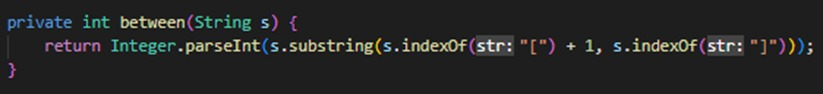
\includegraphics[scale=0.5]{R2.jpeg}    
    \end{center}
    Por \'ultimo, el m\'etodo \code{between( String s )} permite encontrar el id del mensaje que entra por par\'ametro, esto se hacer por medio del m\'etodo substring para extraer una subcadena que comienza justo despu\'es del corchete de apertura y termina justo antes del corchete de cierre.
    (Esto es permitido de acuerdo a la estructura escogida para las transformaciones y producciones de los diversos mensajes).
    Esta subcadena se convierte en un n\'umero entero utilizando el m\'etodo \code{Integer.parseInt( String s )} y se devuelve como resultado.\\

    \subsection{Estructura de Input}
    Tan pronto el usuario corra el programa la consola imprimirá estos tres mensajes secuencialmente: 
    \begin{center}
        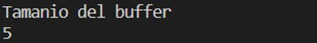
\includegraphics[scale=0.5]{I0.jpeg}    
    \end{center}
    Primero deberá ingresar el tamaño de los buffers, este número deber ser entero y mayor a 0. En este caso es 5. 
    \pagebreak
    \begin{center}
        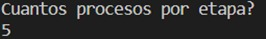
\includegraphics[scale=0.5]{I1.jpeg}    
    \end{center}
    Luego deberá ingresar el número de procesos por etapa, de los cuales se sabe que uno es naranja y los restantes son azules. Este número deber ser entero y mayor a 0. En este caso un proceso sería naranja y cuatro serían azules. 
    \begin{center}
        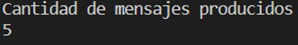
\includegraphics[scale=0.5]{I2.jpeg}    
    \end{center}
    Por último, debe seleccionar la cantidad de mensajes que desea que se produzcan por cada tipo de proceso, este número deber ser entero y mayor a 0. En este caso se producirían 5 mensajes naranjas y 5 azules. 

    Si se desea, también se podría modificar el número de etapas que tiene el programa, sin embargo, por default el número de etapas se estableció como 3. 

    \subsection{Estructura de Prints}
    Al ingresar correctamente los par\'ametros, el programa retornar\'a una estructura de mensajes similar a esta, en donde la ``R'' impresa al inicio significa que por medio del proceso rojo se imprimieron los mensajes.\\
    \begin{center}
        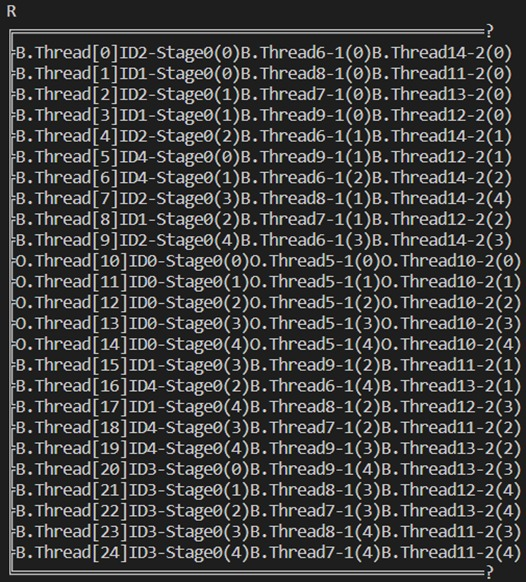
\includegraphics[scale=0.5]{P1.jpeg}    
    \end{center}
    Ahora entendiendo las partes de cada mensaje:
    \begin{center}
        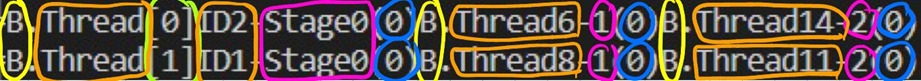
\includegraphics[scale=0.5]{P2.jpeg}    
    \end{center}
    \begin{itemize}
        \item[] Las letras encerradas en c\'irculos amarillos indican el color del proceso por el que pas\'o cada mensaje, si el proceso era azul, la letra representada en el mensaje ser\'a ``B''.\\
        Si el proceso era naranja la letra representada pasa a ser la ``O''.
        \item[] Las palabras se\~naladas en naranja con la estructura ``Thread\#'' siendo \# un n\'umero, representando el id del proceso porque el que pas\'o el mensaje.
        \item[] Los n\'umeros entre llaves encerrados en c\'irculos verdes representan el id de cada mensaje.\\
        Como se puede ver, los mensajes se imprimen conforme al orden otorgado por estos ids.
        \item[] Los n\'umeros encerrados en rosado representan en qu\'e etapa del proceso se realiz\'o cada modificaci\'on.
        \item[] Los n\'umeros entre par\'entesis se\~nalados en azul representan el n\'umero de mensajes que hab\'ia procesado cada proceso hasta ese momento.
    \end{itemize}
    Teniendo en cuenta esto, se puede ver que el mensaje generado cuando se crea el proceso es m\'as espec\'ifico que los que se generan en las etapas posteriores, sin embargo, tienen una estructura que sigue otorgando gran informaci\'on.

    %------------------------------------------------


    \section{Pruebas del programa}

    \subsection{Estructura y requerimientos de prueba}
    Este programa fue probado en el IDE integrado IntelliJ IDEA 2022.3.2, con el JDK Java 11 y en la consola integrada del IDE.
    Fue probado en Windows 10 2H22 y Manjaro Linux 22.10, la estructura del proyecto est\'a planteada con el sistema de Build dbl Java puro y es independiente librer\'ias externas.
    Sin embargo, para conseguir los prints con s\'imbolos integrados, la fuente de la consola en la cu\'al se compile debe ser compatible con simbolos Unicode,
    de lo contrario, solo ser\'a mostrado el c\'odigo Unicode referente a los s\'imbolos.
    Finalmente, solo es una decisi\'on est\'etica.

    \subsection{Pruebas}

    \subsubsection{10-10-10}
    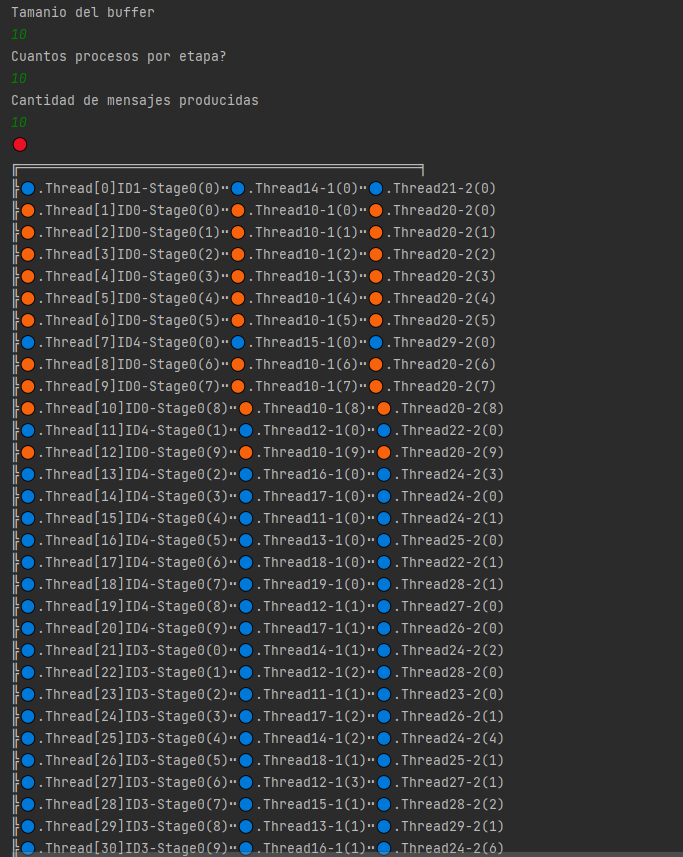
\includegraphics{10-10-10.PNG}

    \subsubsection{3-3-3}
    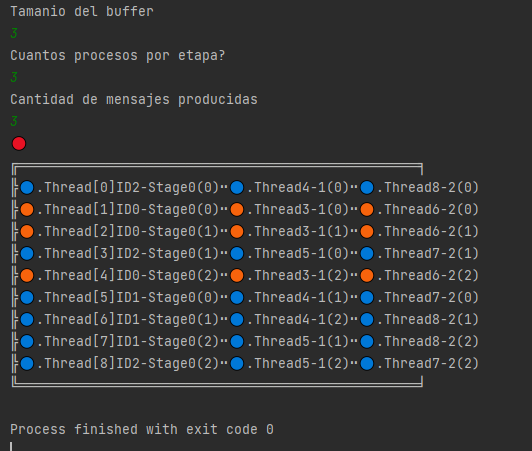
\includegraphics{3-3-3.PNG}

    \subsubsection{5-5-5}
    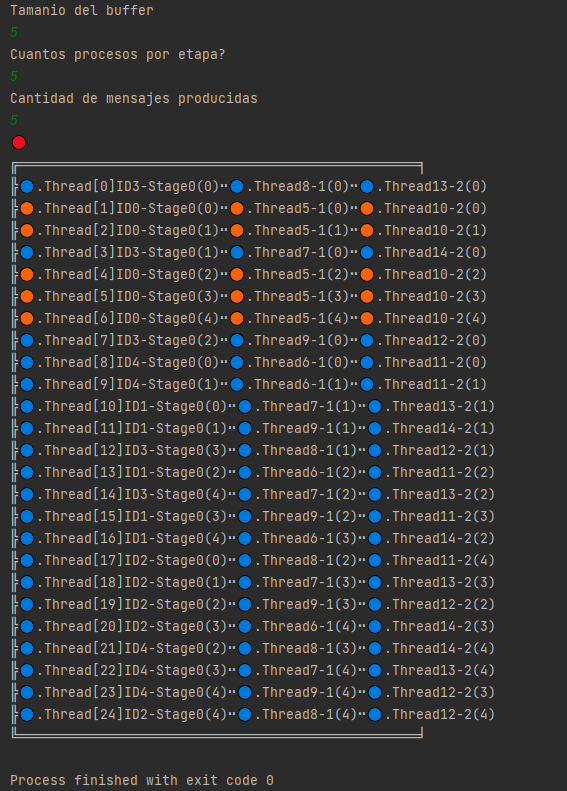
\includegraphics{5-5-5.PNG}


    \section{Glosario}

    \paragraph{Funci\'on Lambda}
    Es una funci\'on an\'onima, es decir, no depende de alguna clase.
    Similar a los m\'etodos toman parametros y retornan alg\'un valor, pero a diferencia de los primeros, estas no necesitan un nombre.
    \paragraph{Objeto an\'onimo}
    Es un objeto que no pertenece realmente a alguna clase, similar a las estructuras en C.
    Como dicho objeto no hace referencia a alguna clase ya declarada, no referencia a alg\'un archivo .java y es principalmente usado para interactuar con bloques de expresiones lambda y si realmente no se considera valioso crear una clase para esta instancia.

%------------------------------------------------
\end{document}
